\section{Opis wykorzystanych technologii}
Realizacja celu pracy wymagała wykorzystania wielu różnych technologii. Zarówno do realizacji aplikacji mobilnej, jak i serwerowej, konieczne było wybranie konkretnych metod. W tym rozdziale zostały one przedstawione oraz szczegółowo omówione.

\subsection{Kody graficzne QR}
Przedstawianie danych w postaci kodów graficznych nie jest niczym innowacyjnym - w sklepach towary oznaczane są za pomocą jednowymiarowego kodu kreskowego. Kombinacja jasnych oraz ciemnych linii umożliwia przechowywanie danych, które odczytywane są za pomocą skanera z laserem. Tego typu metody stosuje się głównie w celach identyfikacji. Do przechowywania większej ilości danych wykorzystuje się częściej tzw. kody 2D.

Kody QR (ang. Quick Respone - szybka odpowiedź) to dwuwymiarowe, kwadratowe kody graficzne. Składają się z modułów, czyli kombinacji ciemnych oraz jasnych kwadratów, które są nośnikami danych. Zostały stworzone przez japońską firmę Denso-Wave w 1994 r \cite{thonky_tutorial}. Według postanowień licencyjnych mogą być wykorzystywane bez żadnych opłat, a sam standard jest opisany w normie ISO/IEC 18004:2015 \cite{norma_qr}. Dzięki dodatkowemu wymiarowi, pozwalają na przechowywanie większej ilości informacji (do ok. 7000 liczb lub 4000 znaków alfanumerycznych) niż kody kreskowe, posiadające tylko jeden wymiar. Ponadto, zapewniają zdecydowanie lepszą korekcję błędów. Nawet częściowo uszkodzony kod może zostać poprawnie odczytany. Posiadają kilka miejsc szczególnych do ułatwienia orientacji podczas odkodowywania. Ich liczba zależy od rozmiaru kodu.

\begin{figure}[h]
	\begin{center}
		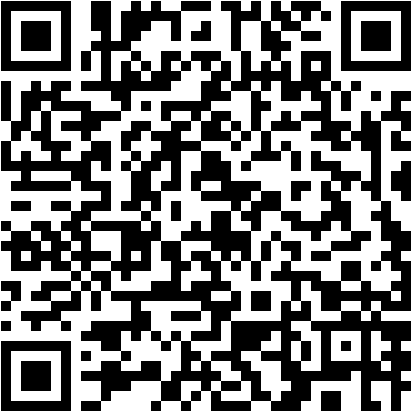
\includegraphics[width=0.2\textwidth]{02/qr_title}
	\end{center}
	\caption{Tytuł pracy przedstawiony w postaci kodu QR}
	\vspace{-0.3cm}
\end{figure}

Pierwotnie bardzo duże zastosowanie kody QR znalazły w logistyce, gdzie zawierały informacje o przesyłanych paczkach. Współcześnie kojarzone są przeważnie z urządzeniami mobilnymi. Spotykane na przystankach, w sklepach lub magazynach służą do komunikacji z użytkownikami smartfonów, przełamując niejako barierę między światem wirtualnym, a rzeczywistym. Kod zawiera informacje jedynie w postaci liczb, liter i symboli. Jednak odpowiednie formatowanie informacji, pozwala na dodatkowe interpretowanie ich przez urządzenie przenośne. I tak po zeskanowaniu może zostać wysłana wiadomość e-mail, albo dodany numer do kontaktów. Najczęściej jednak zawierają adresy URL, które powodują wyświetlenie odpowiedniej strony w przeglądarce internetowej telefonu.

\subsubsection*{Sposoby kodowania}
Przed zakodowaniem informacji do postaci kodu QR, należy określić trzy główne parametry. Są to: wersja, typ danych oraz poziom korekcji błędów.

Najważniejszym parametrem, wpływającym bezpośrednio na ilość danych jakie kod będzie w stanie przechować, to jego wersja. Numerowana jest od 1 do 40 i każda z nich ma przypisany do siebie rozmiar. Wersja pierwsza posiada 21 na 21 modułów, druga 24 na 24, a ostatnia, czyli czterdziesta - 177 na 177. Każda kolejna jest większa od poprzedniej o trzy moduły na bok. Oczywiście im numer wersji, czyli też rozmiar, jest większy, tym więcej danych będzie można zakodować. 

Równie ważne jak wybór wersji jest określenie typu danych, jaki ma być zakodowany. Informacja o typie zapisywana jest w kodzie QR, dzięki czemu podczas odczytywania czytnik wie jak ma interpretować dane. Dodatkowo, ta informacja decyduje też o maksymalnej pojemności. Typ numeryczny przechowuje informacje jedynie o liczbach, dlatego będzie potrzebował mniej bitów na znak, niż w przypadku danych alfanumerycznych. Dostępne są cztery typy:
\begin{itemize}
	\item Numeryczny -- ten tryb pozwala na zakodowanie tylko cyfr od 0 do 9, co umożliwia maksymalnie na przechowywanie 7089 znaków.
	\item Alfanumeryczny -- oprócz cyfr, także wielkie litery oraz znaki '\$', '\%', '*', '+', '-', '.', '/', ':' i spacja. Można zakodować do 4296 znaków. 
	\item Binarny -- domyślnie dla zestawu znaków z ISO-8859-1, ale także UTF-8. Maksymalnie 2953 znaków.
	\item Kanji -- znaki z systemu kodowania Shift JIS. Pomieści nie więcej niż 1817 znaków.
\end{itemize}

Poziom korekcji błędów służy do określenia, czy dane zostały odczytane poprawnie. Pozwala także na odzyskanie części z nich, nawet jeśli kod został uszkodzony (dzięki algorytmowi Reeda-Solomona). Specyfikacja wyróżnia cztery poziomy korekcji. Obok każdego z nich podany został procent danych, jakie można odzyskać:
\begin{itemize}
	\item L (Low) - 7\% danych,
	\item M (Medium) - 15\% danych,
	\item Q (Quartile) - 25\% danych,
	\item H (High) - 30\% danych.
\end{itemize}

\begin{table}[h]
	\caption{Pojemność kodów QR dla różnych ustawień}
	\vspace{0.3cm}
	\begin{center}
		\begin{tabular}{| c | c | c | c | c | c | c |}
			\hline
			Wersja & Moduły & Korekcja & Numeryczny & Alfanumeryczny & Binarny & Kanji\\
			\hline
			\multirow{4}{*}{1} & \multirow{4}{*}{21x21}&L&41&25&17&10\\
			& & M&34&20&14&8\\
			& & Q&27&16&11&7\\
			& & H&17&10&7&4\\
			\hline
			\multirow{4}{*}{40} & \multirow{4}{*}{177x177}&L&7089&4296&2953&1817\\
			& & M&5596&3391&2331&1435\\
			& & Q&3993&2420&1663&1024\\
			& & H&3057&1852&1273&784\\
			\hline
		\end{tabular}
	\end{center}
\end{table}

Tworzenie kodu graficznego QR jest procesem dość złożonym. Po analizie danych określającej ich typ, konieczne jest ich odpowiednie zakodowanie. Informacje dzielone są na bloki, do których dodawane są kolejne bity związane z korekcją błędów. Przed przedstawieniem danych w postaci modułów QR, ważne jest również odpowiednie ich maskowanie. Zbyt duża ilość kwadratów o tym samym kolorze w jednym miejscu, może spowodować błędne odczytanie. Dopiero po tych kilku etapach, może zostać wygenerowany kod. Praktycznie dla każdego języka istnieją biblioteki, które wykonują te wszystkie procesy. Wystarczy podać jedynie parametry kodu z danymi. Na przykład w Pythonie takim modułem jest \textit{qrcode}.

Odczytanie, czyli odkodowanie informacji możliwe jest na wiele sposobów. Razem z systemami mobilnymi często dostarczane są specjalne aplikacje, które wykorzystując wbudowaną kamerę, pozwalają na odczytanie zakodowanych danych. Podobnie, takie rozwiązanie możliwe jest dzięki odpowiednim biblioteką. W Androidzie jest to dostępna za darmo \textit{Zebra Crossing}.


\subsection{System Android}
% o systemach mobilnych. Procentowy udział - wykresik
% Android, krótko co to jest
% Android, krótka historia
% opisać jak to działa pod spodem. Java, kompilacja, Dalvik
Systemy na urządzenia mobilne z czasem stawały się coraz bardziej zaawansowane, przypominając swoją funkcjonalnością te przeznaczone na komputery. Dzisiaj oprócz obsługi podstawowych zadań telefonu, jak dzwonienie, pozwalają na przeglądanie internetu, czy instalowanie dodatkowych aplikacji. Do najpopularniejszych systemów w Polsce należą: Android z 65\% udziałem w rynku, Windows Phone - 16\% i iOS - 4\% \cite{polska_jest_mobi}.


\subsubsection*{O Androidzie}

Android to mobilna platforma systemowa, stworzona w 2003~r, a następnie wykupiona przez Google'a w 2005~r. z rąk niewielkiej firmy Android Inc. Od 2007~r. rozwijany jest w ramach sojuszu kilkudziesięciu firm - Open Handset Alliance. Android został zbudowany na bazie jądra Linuksa, i podobnie jak on rozpowszechniany jest za darmo z dostępnym publicznie kodem. To właśnie dostępność oraz możliwość dowolnego modyfikowania spowodowała, że zdołał w tak niedługim czasie zawładnąć rynkiem, stając się najpopularniejszym systemem mobilnym. Można go spotkać na większości popularnych urządzeń przenośnych, jak: telefony komórkowe, smartfony, tablety, netbooki. Jest stosowany także w e-bookach niektórych firm, czy innych sprzętach domowego użytku. 

%\begin{figure}[h]
%	\begin{center}
%		
\includegraphics[width=0.1\textwidth]{02/android}
%	\end{center}
%	\caption{Logo Androida}
%\end{figure}

\subsubsection*{Architektura systemu}
Ze względu na architekturę systemu, można wyróżnić w Androidzie kilka abstrakcyjnych warstw: aplikacji, frameworku aplikacji, bibliotek, środowiska wykonawczego i jądra Linux, na którym bazuje cały system. Cała funkcjonalność systemu, niezbędna podczas działania aplikacji, dostępna jest poprzez framework aplikacji, czyli systemowe API napisane w Javie. Używając go, programista może kontrolować sposób działania oraz wygląd programu. Tutaj znajduje się menedżer aktywności (ang. Activity Manager), odpowiedzialny za cykl życia aplikacji, czy menedżer powiadomień (ang. Notification Manager) obsługujący wyświetlanie wszelkich notyfikacji. Także udostępnianie przez aplikacje interfejsów, z wykorzystaniem intencji, możliwe jest dzięki tej warstwie. Poniżej jej znajdują się natywne biblioteki, napisane w C i C++. Dzięki systemowemu API najczęściej nie ma konieczności z nich korzystać, i do tworzenia aplikacji można używać Javy. Najgłębiej w systemie znajduje się jego jądro, czyli Linux. Wykonuje ono najbardziej podstawowe funkcje, będąc odpowiedzialnym m.in. za zarządzanie baterią. Posiada też sterowniki systemowe: ekranu, aparatu, czy audio.
\begin{figure}[h]
	\begin{center}
		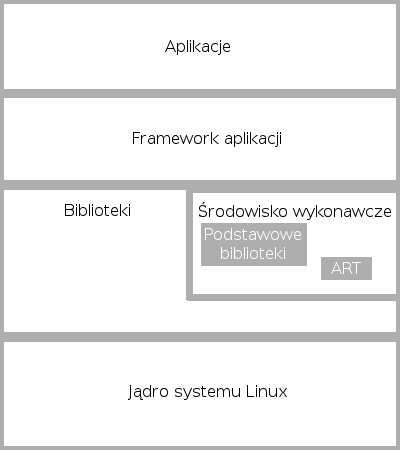
\includegraphics[width=0.5\linewidth]{02/warstwy_android}
	\end{center}
	\caption{Schemat architektury systemu Android}
\end{figure}
\subsubsection*{Środowisko wykonawcze}
Uruchamianiem programów napisanych w Javie zajmuje się wirtualna maszyna Javy (ang. Java Virtual Machine). Po skompilowaniu tworzony jest kod bajtowy, plik \textit{class}, który następnie po załadowaniu interpretowany jest przez JVM (możliwa też kompilacja JIT). Takie podejście pozwala na przenośność programów, czyli niezależność od platformy, kosztem pewnego spadku wydajności.

Mimo, że programy na Androida pisane są w Javie, to nie JVM używany jest do ich późniejszego wykonywana. Głównie jest to spowodowane chęcią stworzenia środowiska uruchomieniowego, które będzie lepiej przystosowane do słabszych wydajnościowo od komputerów maszyn, jakimi są urządzenia mobilne. Proces budowania aplikacji rozpoczyna się tak samo. Kompilator przekształca pliki zawierające kod Javy, do kodu bajtowego. W takiej postaci program nie mógłby zostać jeszcze uruchomiony. Najpierw specjalne narzędzie, pod nazwą \textit{dx}, modyfikuje wynik działania kompilatora. Dla każdej klasy Javy tworzony jest osobny plik \textit{class} - w trakcie działania programu są one ładowne przez JVM. Zadaniem \textit{dx} jest połączenie wszystkich tych kodów bajtowych w jeden plik \textit{dex}, z usunięciem powtarzających się symboli oraz zmianą znajdujących się tam instrukcji, na odpowiednie dla Androida. Dzięki temu skompilowany program będzie mniejszy oraz powinien działać szybciej. Ostatnim etapem budowania aplikacji jest stworzenie pliku \textit{apk}, odpowiednika \textit{jar}, w którym oprócz kodu bajtowego, znajdą się takie zasoby jak zdjęcia wykorzystywane w aplikacji.
\begin{figure}[h]
	\begin{center}
		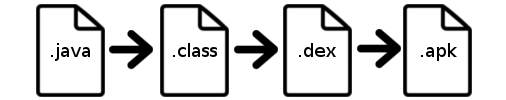
\includegraphics[width=0.5\textwidth]{02/android_dex}
	\end{center}
	\caption{Proces budowy aplikacji}
	\vspace{-0.5cm}
\end{figure}

Do wersji 4.4 Androida (KitKat) aplikacje uruchamiane były w wirtualnej maszynie Dalvik. Sposób działania jest dość zbliżony do JVM. Kod bajtowy w postaci plików \textit{dex} jest interpretowany, z możliwością kompilacji do kodu natywnego (JIT). Jedną z różnic jest sposób działania wirtualnego procesora, który w Dalviku opartu został na rejestrach, a nie na stosie. Takie podejście wpływa na mniejsze zużycie pamięci, jednak programy są większe, gdyż instrukcje muszą zawierać dodatkowe informacje co do rejestrów, z których korzystają.

W wersji 5.0 Androida (Lolipop) zastąpiono dotychczasową maszynę wirtualną Dalvik, środowiskiem uruchomieniowym Android runtime (ART). Również przyjmuje pliki \textit{dex}, jednak nie interpretuje ich, a w momencie instalacji aplikacji - kompiluje. Taka kompilacja kodu pośredniego, języka wysokiego poziomu, do kodu natywnego, nosi nazwę Ahead-of-time (AOT). Przy każdym uruchomieniu aplikacji, dzięki ART, wykorzystywany jest jej natywny kod. Ta zmiana powoduje szybsze działanie i uruchamianie się aplikacji. Wadą jest znacznie dłuższy czas instalacji, który teraz obejmuje także dodatkową kompilację.


\subsubsection*{Programowanie aplikacji}
Aby móc tworzyć aplikacje na Androida z wykorzystaniem Javy, konieczne jest posiadanie:
\begin{itemize}
	\item Java z JDK i JRE,
	\item Android SDK.
\end{itemize}
W ten sposób aplikacja do funkcji systemowych odwoływać się będzie za pomocą udostępnionego przez system API, przeznaczonego dla Javy. Dzięki temu, że nie jest to kod natywny, nie jest konieczna osobna kompilacja dla każdej dostępnej architektury. Programy są uniwersalne i dopiero po zainstalowaniu na konkretnym urządzeniu, interpretowany jest kod bajtowy, bądź przeprowadzana kompilacja AOT. Przez twórców systemu udostępniane jest NDK, czyli Native Development Kit. Z jego pomocą aplikacje mogą być tworzone w C lub C++, odwołując się bezpośrednio do bibliotek systemowych. Niestety, mimo możliwego zysku na wydajności, stworzony kod jest zależny od architektury. Dodatkowo większość zewnętrznych bibliotek jest tworzonych w Javie. 

Bardzo zalecane jest używanie zintegrowanego środowiska programistycznego, które automatyzuje niektóre czynności. Potrafi stworzyć za użytkownika projekt z wymaganą strukturą plików, wykonać wszystkie etapy kompilacji, wgrać program na urządzenie i wiele innych. Dedykowanym IDE jest Android Studio, do niedawna wykorzystywany był domyślnie Eclipse.

\begin{figure}[h]
	\begin{center}
		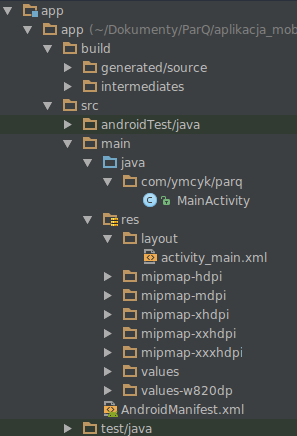
\includegraphics[width=0.25\textwidth]{02/android_pliki}
	\end{center}
	\caption{Pliki projektu utworzonego w Android Studio}
	\vspace{-0.3cm}
\end{figure}
Podczas działania aplikacja prezentuje użytkownikowi tzw. ekrany. Są to odpowiedniki okien systemowych, gdzie umieszczane są elementy graficznego interfejsu użytkownika, czyli widoki (ang. views), jak np.: przyciski, rozwijane listy, czy pola tekstowe. Wchodząc z nimi w interakcję (poprzez dotyk, w ekranach dotykowych), możliwa jest komunikacja między użytkownikiem, a urządzeniem. 

Wygląd ekranów definiowany jest w plikach XML, nazywanych układami (ang. layout). Każdy z widoków jest osobnym znacznikiem, a za pomocą argumentów można modyfikować wybrane parametry jak rozmiar, czy kolor. Wszystkie widoki w pliku XML muszą posiadać swojego rodzica, który definiuje jak mają one być traktowane w tym układzie. W Androidzie można skorzystać z trzech. RelativeLayout - położenie widoków określane jest względem siebie. LinearLayout - układ liniowy, gdzie elementy GUI wyświetlane są jeden koło drugiego. GridLayout - dzieli ekran na siatkę, składającą się z wierszy oraz kolumn, i pozwala umieścić widoki we wskazanych komórkach.

Układy definiują jak dany ekran ma wyglądać, natomiast aktywności (ang. activity), czyli klasy Javy, określają w jaki sposób mają one reagować na interakcje użytkownika. Przechodząc do danego ekranu, tworzona jest najpierw aktywność. W metodzie onCreate, wywoływanej przed wyświetleniem ekranu, wybierany jest układ, który ma zostać użyty przez system do stworzenia interfejsu. Widoki z tego układu mogą mieć powiązane ze sobą jakieś operacje, które będą przeprowadzane np.: po naciśnięciu przycisku. To także odbywa się w aktywności, która może posiadać metody wywoływane po zakończeniu danej interakcji.

\subsubsection*{Podsumowanie}
Rozwiązania mobilne cieszą się coraz większym zainteresowaniem. Tylko w sklepie z aplikacjami Androida, Google Play, liczba programów przekroczyła w 2015 r. 1,6 mln \cite{biblia_ebiznesu_2}. Powstające coraz to nowe urządzenia, na których zainstalowany jest Android sprawia, że umiejętność programowania na tą platformę będzie coraz bardziej doceniana.


\subsection{Framework Django}
Frameworki aplikacji internetowych powstały z myślą o zwolnieniu programisty z obowiązku pisania części kodu, który jest wspólny dla większości serwisów. Może to być dostęp do bazy danych, obsługa linków (ang.~routing), czy zarządzanie sesjami. Dodatkowo, pisanie aplikacji internetowej od podstaw, jest zadaniem czasochłonnym oraz dość trudnym. Frameworki są odpowiedzią na te problemy, dostarczając zestaw gotowych oraz przetestowanych rozwiązań, które należy dostosować do własnych potrzeb. Umożliwiają utworzenie struktury plików projektu, na bazie którego dalej będzie rozwijana aplikacja. Każdy z najpopularniejszych języków programowania oferuje duży wybór silników, przeznaczonych do tworzenia usług internetowych i np.: w C\# napisane zostały ASP.NET i MonoRail, w Javie - Spring i JavaServer Faces, a w Python - Django i Flask. Mogą się różnić przede wszystkim stopniem złożoności, dzięki czemu nadają się do różnych zastosowań - prezentują odmienne sposoby realizacji podobnych zadań. Wybór programisty będzie głównie zależny od jego prywatnych preferencji.

\subsubsection*{Początki Django}
Django rozwijany jest jako wolne oprogramowanie na GitHub'ie, w ramach fundacji Django Software Foundation, ale skupiaja wokół siebie także wielu niezależnych twórców. Został napisany w Pythonie, stając się z czasem najpopularniejszym frameworkiem dla tego języka. Jego historia rozpoczęła się w 2003~r., kiedy to dwóch programistów Adrian Holovaty i Simon Willison zaczęli używać Pythona do tworzenia aplikacji webowych dla kilku serwisów informacyjnych, m.in. Lawrence.com. Praca w środowisku dziennikarskim, cechująca się napiętym grafikiem, wymagała niezwykle szybkiej realizacji zadań. Z tej konieczności opracowali własny silnik, który w 2005~r., już pod nazwą Django, został udostępniony publicznie. To właśnie szybkość oraz względna łatwość tworzenia aplikacji są jego głównymi zaletami.

\subsubsection*{Charakterystyka}
% trochę upośledzone MVC
% diagram 
% zabezpieczenia
% admin
% modele
% o dodatkach parę słów
Aplikacje Django tworzone są w interpretowanym języku Python, przeznaczonym głównie do pisania skryptów. Jako że jego interpretery dostępne są na wielu platformach, jest on niezależny od systemu operacyjnego. Dodatkowo wsparcie do wielu paradygmatów (imperatywnego, funkcyjnego, obiektowego), przekłada się na jego szerokie zastosowanie. Oprócz programowania serwerów, jest używany do pisania testów, aplikacji z graficznym interfejsem, a także gier 3D. Wyróżnia się głównie charakterystyczną składnią, w której poszczególne bloki kodu odseparowane są wcięciami (spacje lub tabulator). Wpływa to na zwiększoną czytelność kodu.

Architektura aplikacji sieciowych typu klient-serwer, opiera się często na wzorcu projektowym Model-View-Controller (pol.~Model-Widok-Kontroler), w skrócie MVC. Jego ideą jest odseparowanie części prezentacji danych, od kodu odpowiedzialnego za ich przetwarzanie. Aplikacja dzielona jest w nim na trzy główne części. Model jest reprezentacją danych oraz logiki problemu. Widok odpowiedzialny jest za prezentację - określa w jaki sposób informacje mają zostać przedstawione. Kontroler przyjmuje żądania i wykonuje związane z nimi akcje. Głównie aktualizuje widoki oraz modele.

\begin{figure}[h]
	\begin{center}
		\includegraphics[width=0.6\textwidth]{02/MVC_diagram}
	\end{center}
	\caption{Wzorzec projektowy MVC}
	\vspace{-0.3cm}
\end{figure}

Wzorzec MVC jest stosowany w Django, jednak został zrealizowany w sposób odmienny od najczęściej spotykanych jego implementacji. Z tego względu często nazywa się go wzorcem MTV (Model-Template-View), będącego pewną wariacją MVC. Także wyróżnia się w nim trzy główne części aplikacji, a są to:
\begin{itemize}
	\item Model -- podobnie jak w MVC, zapewnia dostęp do danych. Opisane są tutaj relacje między danymi oraz odbywa się ich walidacja.
	\item Template (pol. szablon) -- warstwa prezentacji, czyli jak ma zostać wygenerowana odpowiedź (w postaci dokumentu HTML lub innym formacie).
	\item View (pol. widok) -- zawiera logikę biznesową. Pobiera dane z modeli i łączy je z szablonami, tworząc w ten sposób odpowiedź. Stanowi pomost między dwoma wcześniej wymienionymi elementami MTV.
\end{itemize}
Rolę kontrolera MVC pełni w Django sam framework. Otrzymane zapytanie wysyłane jest do odpowiedniego widoku, w zależności od konfiguracji URL.
\begin{singlespace}
	\captionof{listing}{Przykładowa konfiguracja URL w Django}
	\vspace{0.3cm}
	\inputminted[fontsize=\footnotesize]{python}{src/urls.py}
	\label{l:url}
\end{singlespace}

% tutaj o wszystkich cechach Django
W przeciwieństwie do mikro frameworków, takich jak Flask, Django dostarcza programiście wielu gotowych rozwiązań, jak: dostęp do baz danych, klasy ORM, obsługa linków URL, uprawnienia użytkowników, automatycznie generowana strona administratora, szablony HTML i wiele innych. Dodatkowo posiada wbudowaną ochronę przed typowymi atakami, takimi jak: cross-site scripting (XSS), cross-site request forgery (CSRF), a także wstrzykiwanie SQL'a.

\subsubsection*{Programowanie aplikacji}
Tak jak większość frameworków, także i Django tworzy za użytkownika gotową strukturę projektu. Poza konfiguracją, nie znajduje się w nim jednak żadna logika. Wszystkie modele oraz widoki w danym projekcie tworzone są w ramach tzw. aplikacji, czyli pakietów Pythona (których struktura także generowana jest przez framework), odpowiednio w plikach models.py oraz views.py. Dzięki temu mogą zostać one ponownie wykorzystane. W hierarchii plików znajdują się na tym samym poziomie, co projekt. 
\begin{figure}[h]
	\begin{center}
		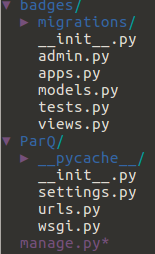
\includegraphics[width=0.15\textwidth]{02/django_structuree}
	\end{center}
	\caption{Struktura plików projektu (ParQ) z aplikacją (badges)}
	\vspace{-0.3cm}
\end{figure}

W pliku settings.py projektu znajdują się wszystkie ustawienia serwisu, takie jak konfiguracja bazy danych, strefy czasowej, silnika szablonów oraz pakietów pośredniczących (middleware) wykorzystywanych np.: do autoryzacji. Tam także powinny zostać zarejestrowane wszystkie aplikacje używane w projekcie.

W models.py aplikacji znajdują się modele danych - są to klasy dziedziczące po Model. Posiadają zmienne klasowe, które reprezentują kolumny w tabelach baz danych. Nazwa takiego pola jest później używana jako nazwa kolumny, natomiast jej typ definiowany jest przez instancję jednej z klas pochodnych od Field. I tak dla przykładu IntegerField będzie typem całkowitoliczbowym, a CharField znakowym. Parametry podane w konstruktorze pozwalają zdefiniować rozmiar, czy unikalność krotki w kolumnie. Relacje również tworzone są za pomocą pól. Model posiadający pole relacji, może odwoływać się za jego pomocą do powiązanych danych. W Django znajdują się trzy takie klasy:
\begin{itemize}
	\item ForeignKey -- pole z kluczem obcym, używane w relacjach jeden do wielu. Tworzona jest kolumna w tabeli.
	\item ManyToManyField -- używane w relacjach wiele do wielu. W bazie danych zostanie automatycznie utworzona tabela pośrednia, z kluczami powiązanych tabel.
	\item OneToOneField -- do relacji jeden do jeden. Także wykorzystywana jest tabela pośrednia, jednakże oba klucze są unikalne - mogą wystąpić tylko w jednej relacji w ramach tej tabeli.
\end{itemize}

W modelach dozwolone jest także definiowanie własnych metod.

\begin{singlespace}
	\captionof{listing}{Przykładowy model danych z modułu models.py}
	\vspace{0.3cm}
	\inputminted[fontsize=\footnotesize]{python}{src/models.py}
\end{singlespace}

Kolejnym ważnym plikiem w aplikacji tworzonej przez użytkownika jest views.py. To tutaj znajdują się widoki ze wzorca MTV i scalają one szablony z modelami. Jako parametr przyjmują obiekt HttpRequest, zawierający dane zawarte w żądaniu HTTP. To właśnie te widoki podawane są podczas konfiguracji linków w funkcji url, pliku urls.py w projekcie. Zostało to zaprezentowane na listingu \ref{l:url}.

\begin{singlespace}
	\captionof{listing}{Widok}
	\vspace{0.3cm}
	\inputminted[fontsize=\footnotesize]{python}{src/views.py}
\end{singlespace}

\subsubsection*{Aplikacje jako dodatki}
Napisane aplikacje Django, mogą być wielokrotnie wykorzystywane w innych projektach. Na tej zasadzie funkcjonują dodatki pisane do tego frameworku. Jednymi z nich są: Django REST Framework używany do tworzenia API w architekturze REST, czy django-annoying modyfikujący działanie niektórych elementów silnika.

%\begin{listing}[H]
%	\caption{Kod powyżej}
%	\vspace{0.5cm}
%	\inputminted[fontsize=\footnotesize]{python}{src/models.py}
%\end{listing}
